\chapter{Work Done}
 
\section{First work}

During the first month, my work was mainly focused on being familiar with the
project and the data, in order to find the best way to contribute to the project.

\subsection{Python library}

Carmine Carratù, the previous ERASMUS student, has been working on algorithms for the
computation of distance transform into $G-maps$. My goal was to understand the code
and know how to use it to create figures for future publications. The code was not
documented so in reading the code I started to comment it and create documentation.
I also bring some optimizations to the code. Some functions was not very helpful for
the purpose of the project and the code was in several files, whereas we wanted to
keep the code as simple as possible in one notebook. So I created this notebook to
combine all the usefful and documented functions in one place.

\subsubsection{New representation on a $G-map$}

\begin{figure}
    \centering
    \begin{subfigure}{0.49\textwidth}
        \centering
        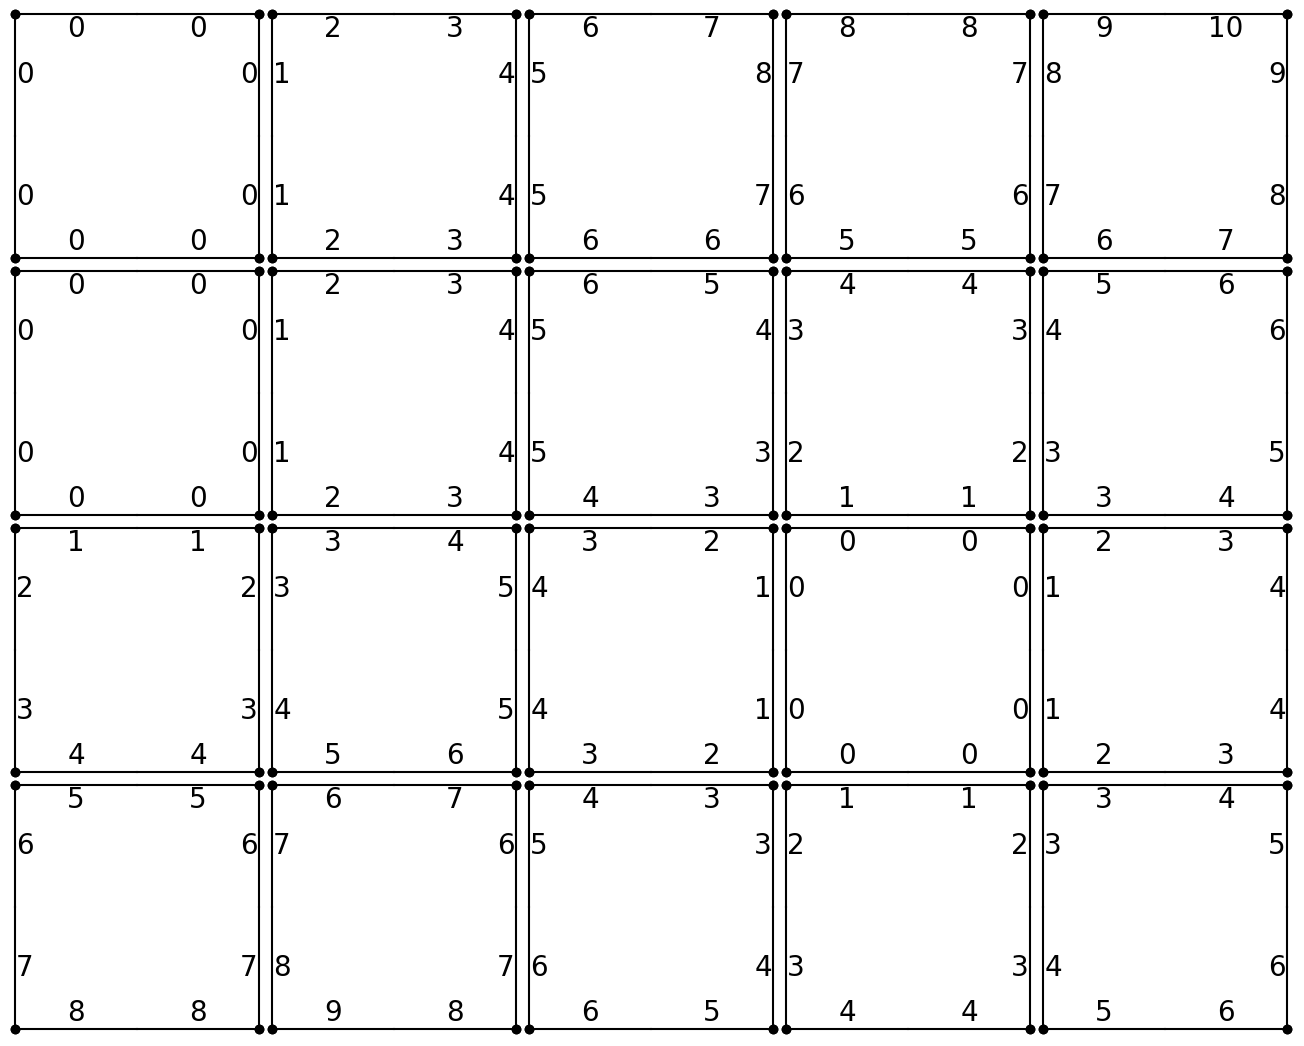
\includegraphics[width=\textwidth]{figures/gmap_dt_old.png}
        \caption{Old representation}
        \label{fig:gmap_dt_old}
    \end{subfigure}
    \hfill
    \begin{subfigure}{0.49\textwidth}
        \centering
        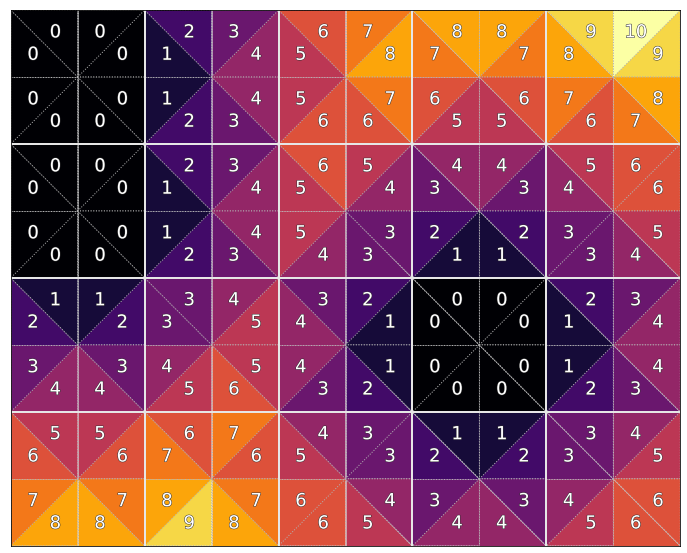
\includegraphics[width=\textwidth]{figures/gmap_dt_new.png}
        \caption{New representation}
        \label{fig:gmap_dt_new}
    \end{subfigure}
    \caption{Different representations of the distance transform on a $G-map$}
    \label{fig:gmap_dt}
\end{figure}

The representation of the distance transform was changed to be more intuitive. On
the figure (\ref{fig:gmap_dt_old}) the distance transform is represented as a
$G-map$ with the distance values on the dart. It's hard to see the variation of the
distance values. The new representation is shown in the figure (\ref{fig:gmap_dt_new}).
This representation uses triangles for each dart showing the distance values. In
addition, we use the \textit{inferno} color map that is perceptually uniform with 
monotonically increasing luminance \cite{Moreland}.

\subsubsection{New representation on a leaf image}

\begin{figure}
    \centering
    \begin{subfigure}{0.45\textwidth}
        \centering
        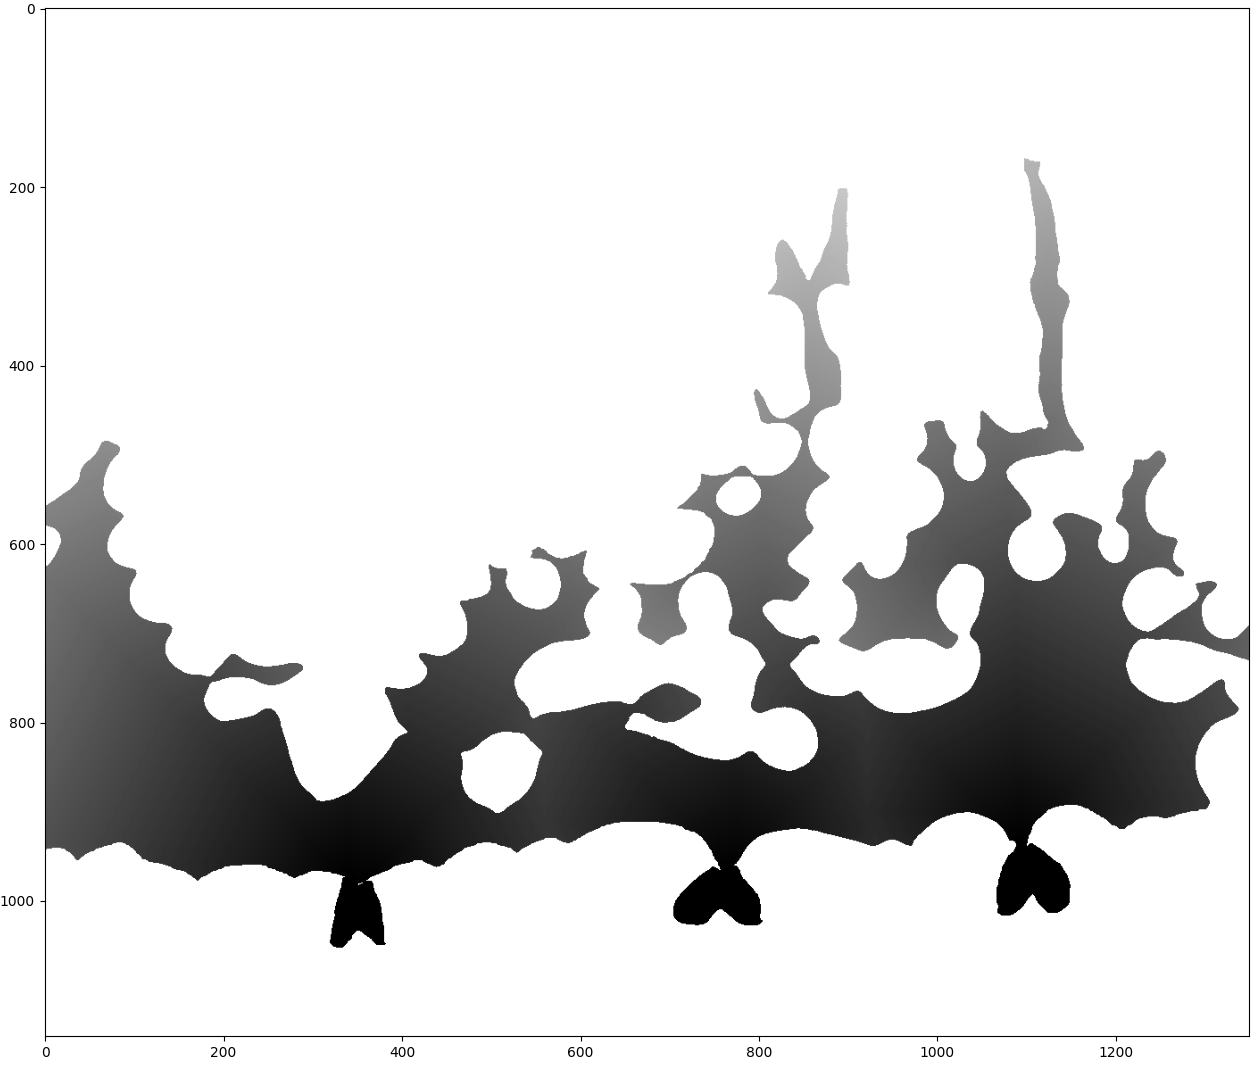
\includegraphics[width=\textwidth]{figures/leaf_dt_old.png}
        \caption{Old representation}
        \label{fig:leaf_dt_old}
    \end{subfigure}
    \hfill
    \begin{subfigure}{0.54\textwidth}
        \centering
        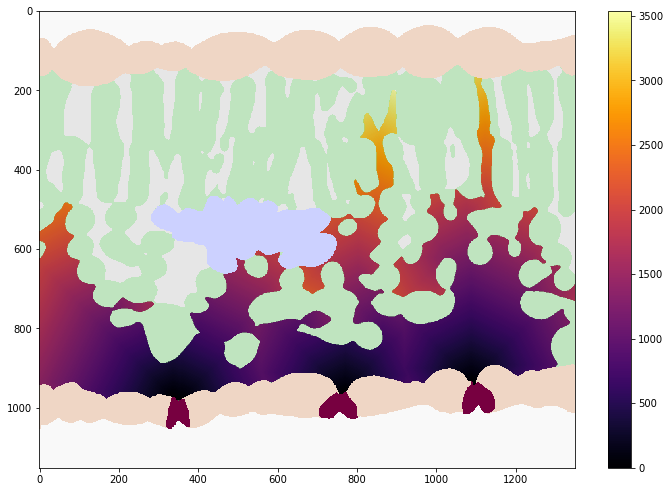
\includegraphics[width=\textwidth]{figures/leaf_dt_new.png}
        \caption{New representation}
        \label{fig:leaf_dt_new}
    \end{subfigure}
    \caption{Different representations of the distance transform on a leaf}
    \label{fig:leaf_dt}
\end{figure}

On the leaf image, the representation was changed too. Before the distance transform
was print with a black and grey color map as shown in the figure (\ref{fig:leaf_dt_old}). 
The new representation, shown in the figure (\ref{fig:leaf_dt_new}) uses the 
\textit{inferno} color map and an overlay can be seen to show the other parts of the 
leaf image.

\subsubsection{Wave propagation animation}

The distance transform algorithm uses a wave propagation method to propagate the
distance values. I used \textit{Click} \cite{CLICK} Python package to create a
command line program that can be used to animate the propagation of the distance
transform.

\subsection{Diffusion equation}

In order to achieve the main goal of the Watergate project it's important to study the
gas exchange process that occurs in plant leaves. The distance transform is used to
compute the geodesic distance from stomata to mesophyll cells where the photosynthesis
is performed. The gas exchange rate depends on this distance over which the diffusion 
occurs \cite{RSB}. To study gas exchanges inside leaves, we have chosen the diffusion
equation, described in 2D by this Partial Differential Equation (PDE):

\begin{equation}
  \frac{\partial u}{\partial t} = \alpha \left( \frac{\partial^2u}{\partial x^2} + \frac{\partial^2u}{\partial y^2} \right)
  \label{eq:heat}
\end{equation}

where $u(x,y,t)$ is the concentration at position $x$, $y$ in time $t$ and $\alpha$ is the
diffusion coefficient.

With a finite-difference method, we can convert the PDE \eqref{eq:heat} into an explicit 
equation described as follows:

\begin{multline}
    u(x,y,t+1) = u(x,y,t) + \alpha \big(
        u(x+1,y,t) + u(x-1,y,t) \\
        + u(x,y+1,t) + u(x,y-1,t) 
        - 4 u(x,y,t)
        \big)
    \label{eq:iterative}
\end{multline}

where $\Gamma(x)$ is the set of neighbors of pixel $x$.
